\chapter{Introduction}
\section{Electronic voting}
Since 2015, it is possible for Swiss citizens registered in the cantons Geneva and Neuchâtel and living abroad, to vote electronically. However, these systems did not yet meet the requirements in terms of security and transparency, to be accepted as a secure E-Voting platform on a nationwide scale.

An e-voting system must satisfy a large variety of security requirements, including but not limited to:

\begin{itemize}
	\item Fairness: It is not possible for any person (including the participating parties of an e-voting system) to learn the intermediate result or outcome of an election before the result has been officially tallied and published to a public board.  
	\item Privacy: No one can find out information about a voters selection. This implies that a voters selection must be encrypted until the election is tallied.
	\item Authenticity: All voters must be authenticated as eligible voters in order to cast a vote
	\item Soundness: Only valid votes are being tallied. If a voter selects more candidates than he is allowed or less than he is supposed to, the vote must not be counted.
 \item Robustness: An e-voting system detects cheating actors.
\end{itemize}

There are many different existing concepts and e-voting protocols that cover most of these requirements. However, most of the existing solutions can be seen as some kind of blackbox, which keep the internals remain hidden, such that a voter cannot be sure, whether his vote has been recorded correctly and counted in the result. 

One of the requirements that is hardest to achieve is the \textbf{universal verification}: A good e-voting system must be transparent and allow an external person to verify, that every protocol participant has abided by the protocol and that all and only valid votes have been counted correctly.

Another common problem is the \textbf{insecure platform problem}: If a voters computer is affected by malware, the vote casting process is no longer under the voters control and the candidate selection could be possibly manipulated without the voters notice. It must be \textbf{individually verifiable} to every voter that his intended vote has been recorded, while at the same time, the voters privacy must still be ensured at all times. 

\section{The CHVote protocol}
%The protocol our project is based on, does not originate from us! The concept and specification has been created by  of the Institute for Security in the Information Society (RISIS) of the Bern University of Applied Sciences. For this project, we have implemented the protocol according to their specification. In this section we summarize the most important aspects of the protocol and establish the terminology for better understanding this document and our application.%
Some of the presented requirements might sound as a paradoxon. However, they can be solved by modern cryptography. A contract was formed between the state of Geneva and the the Institute for Security in the Information Society (RISIS) of the Bern University of Applied Sciences to work out a new protocol which does meet the complex requirements set up by the government. In 2017, Rolf Haenni, Philipp Locher and Reto E. Koenig published the resulting specification document and a proof-of-concept has been successfully implemented by the State of Geneva. Our project is based on this specification. In this section we summarize the most important aspects of the protocol and establish the terminology for better understanding this document and our application. We would like to point out, that the following ideas do not originate from us!

\subsection{Actors}
A \textbf{voter} is a person who is eligible to vote in his respective state. Every voter is assigned a \textbf{counting circle} which typically corresponds to the voters municipal and is required for statistical purposes. For authentication purposes, every voter must possess a voting card that has been sent to him prior to an election event that contains codes used to identify the voter during the vote casting process.

The \textbf{Election Administrator}, typically a person of the government, is responsible for setting up the election event by providing the required information such as the candidates or the voters and initiates the generation of the cryptographic electorate data. He is also responsible for tallying the election and publishing the final results.

The \textbf{election authorities} can be seen as some kind of independent election observers. In a CHVote election event there are always multiple election authorities in order to avoid having to trust a single authority. The authorities are involved in almost every step of the protocol, starting from the generation of their shares of the electorate data, checking and responding to new ballots, as well as in the mixing (a measure to ensure anonymity) and decryption phases. The public key that is used for encrypting the ballots has been jointly generated by all election authorities. Therefore in order to decrypt the ballots, all authorities must work together and provide their share of the private key. 

The measure of multiple authorities participating in the whole e-voting process establishes a \textbf{distribution of trust} and ensures security of the whole election process as long as at least one election authority can be trusted.

The \textbf{Bulletin Board} acts as a central board over which most communication is done and where all the public data is stored. By publishing all non-secret data onto a public board, including the list of encrypted ballots, the protocol is making a big step towards the demanded transparency.

The \textbf{Printing Authority} is responsible for printing the voting cards for all voters. Since the printing authority needs to be in possession of all the secret voting codes, it is a very sensitive point in the protocol. The printed voting cards are handled over to a trusted mailing service for delivery.

\subsection{Pre-Election \& Voting cards}
Before the actual election phase, the vote administrator sets up the election event by entering all required parameters, including the voters, the elections with their corresponding candidates and the number of candidates a voter can select in every election. All election authorities jointly generate the cryptographic data for the whole electorate from which the voting card information is derived. The printing authority combines the information from all election authorities, prints the voting cards and delivers them to the voters by a trusted mailing service. 

A voting card contains several codes, namely:

\begin{itemize}
	\item a voting code
	\item a confirmation code
	\item a finalization code
	\item one verification code for every candidate
\end{itemize}

The \textbf{voting and confirmation codes} are authentication codes and are used to authenticate the voter twice during the vote casting process; the first time with the voting code when he casts his vote, and a second time for confirming his vote. A second authentication code is required because otherwise an attacker who infected a voters computer with malware could just confirm a vote on behalf of the voter after he manipulated the candidate selection and could therefore skip the whole verification process.

\subsection{Vote casting with oblivious transfers}
As mentioned earlier, one of the big challenges of an evoting-protocol is how it deals with the insecure platform problem: A voting platform that is infected with malware poses the risk that an attacker can manipulate the candidate selection on the vote-casting page after the voter has entered his voting code. 

The CHVote specification suggests a "`Cast-as-intended verification"'-step to allow voters to detect this kind of manipulation: When a voter enters his voting code and the indices of his favored candidates, the voting client forms a \textbf{ballot} containing the voters selection encrypted with the authorities public key, his public voting credential derived from the voting code, and a \textbf{non-interactive zero knowledge proof} which proofs that the voter has formed the ballot according to the protocol and that he has been in knowledge of his voting code, without revealing any information about the voting code.

Every election authority has to check the voters public voting credential, the validity of the ballot proof and that the voter hasn't already cast a vote. The encrypted selection also serves as a query for an oblivious transfer. A \textbf{k-out-of-n oblivious transfer} allows a client to query a server for $k$ messages, without the server knowing what messages the client requested, and without the client learning anything about the other $n-k$ messages. Adapted to the CHVote protocol: The voting client queries the authorities for the corresponding verification codes of the selected candidates, without the authorities learning which candidates the voter has selected, and without revealing any information about the other candidates. 

The voter then checks if the returned verification codes match the codes of the candidates he has chosen on the printed voting card. If the selection was somehow manipulated by malware, the returned verification codes would not match the printed ones and the voter would have to abort the vote casting process. This way the integrity of the vote casting process can be guaranteed even in the presence of malware. In such a case, privacy on the other hand cannot be protected since the malware will learn the plaintext of the voters selection.

Another feature the protocol supports, is that an election event can consist of $t$ multiple parallel elections. In such cases, the voter has to submit a single ballot, which contains his candidate selection for all parallel elections. This raises the question, how the system can verify that a voter has chosen exactly the correct number of candidate in each election, and not for example one less in the first, and one additional candidate in the second election.

The specification suggests the following trick: Assuming an election consists of two parallel elections ($t=2$) with 3 candidates each ($n_1 = 3, n_2 = 3$), of which a voter can select one candidate in each election ($k_1 = k_2 =1$). The verification codes are derived from $n = \sum_{j=1}^{t} n_j$ random points on $t$ polynomials (one for every election event $j$) of degree $k_j - 1$, that each election authority has chosen randomly prior to the election. By learning exactly $k = \sum_{n=1}^{t} k_j$ points on these polynomials, the voting client is able to reproduce these polynomials and therefore is able to calculate a particular point with $x=0$ on these polynomials. The corresponding $y$ values are incorporated into the second credential from which the confirmation code is derived. As a result, only if a voter has been able to reconstruct these polynomials with the returned points by submitting a valid candidate selection, he will be able to confirm the vote that he casted.

\subsection{Anonymity with mixnets/cryptographic shuffles}

Since there is still a connection between the encrypted ballot and the voter at this point, the encrypted selections are extracted from the ballots as the first step of the post-election phase. In order to anonymize the list of encryptions, every authority performs a cryptographic shuffle with a random permutation and re-encrypts all ciphertexts in order to make it impossible to find out which voter has submitted which encrypted ballot. This is done by using the multiplicative homomorphic property of the ElGamal encryption scheme. A \textbf{multiplicative homomorphic encryption} scheme allows to perform multiplications on the ciphertext such that:

\begin{equation*}Enc(a) \cdot Enc(b) = Enc(a \cdot b)\end{equation*}

The specification suggests multiplying the encryption with the encryption of the neutral element $1$ since this yields a new ciphertext for the exact same plaintext.

\begin{center}
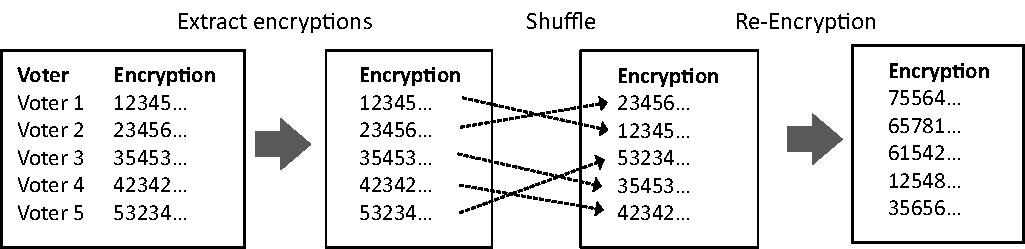
\includegraphics[scale=0.95]{assets/mixing.pdf}
\captionof{figure}{Mixing}\label{Mixing}%
\end{center}

While the extraction only needs to done by the first election authority, every election authority is sequentially performing the shuffle and re-encryption on the mixed list of the previous election authority.

To prevent election authorities from cheating and not performing the mixing the way it is supposed to, a zero-knowledge proof is calculated which will be verified by all election authorities before decryption. If one of these \textbf{shuffle-proofs} fails, the election process can not proceed.

\section{Project task}
An additional problem e-voting is confronted, is that understanding such a complex protocol isn't easy without good knowledge in cryptography and group theory. This might be one of the reasons why many people still do not trust electronic voting systems. 

In close consultation with the authors of the CHVote specification, we were looking for an interesting project for our bachelor thesis. We decided to study the CHVote specification, implement the protocol and build an application that allows to get a hands-on experience with the CHVote e-voting system and that could be used to show and explain to an audience how the future of voting in Switzerland might possibly look like.

\begin{center}
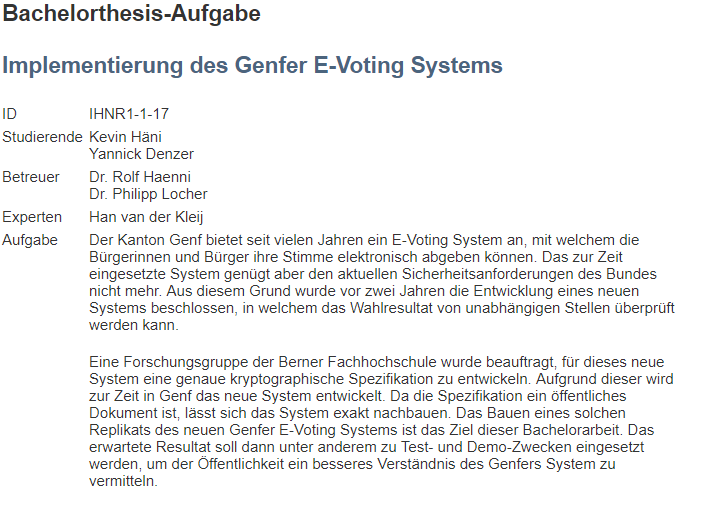
\includegraphics[scale=0.95]{assets/aufgabe.PNG}
\captionof{figure}{Bachelor thesis task}\label{Bachelor thesis task}%
\end{center}

Our project task required us to read and get a good understanding of the CHVote specification. As preparatory work during the course "`Project 2"', which we have finished just before the start of our bachelor thesis, we have implemented the approximately 65 algorithms which were defined as pseudo-code in the CHVote specification document. The resulting set of algorithms has been used as a library for implementing the protocol on which our application will be built on.

Based on this rather general task description, there were several possibilities regarding the final product, such as a realistic prototype, a verifier software for the prototype which was implemented in Geneva, or a demonstrator-application that approaches the educational problem. 

Ultimately we have decided to develop a web-based application which allows to visualize every step of a CHVote election event, from generating the electorate data, to casting and confirming ballots from a voters point of view, to the post-election processes like mixing, decryption and tallying. Opposed to a realistic prototype, the focus on our project is not to implement an e-voting-system that is totally realistic, but more on the visualization.  

The authors of the specification have the intention of using our application for future demonstrations of their protocol to achieve a clearer understanding and better acceptance of e-voting.

In chapter 2, we will further discuss the goals and requirements that we have set for this project. Additionally, it covers the time planing and project methodology and a short (non-technical concept) of our product.

Chapter 3 explains the technical aspects regarding the implementation, such as the architecture, the language and technology decisions. Later sections contain detailed information about the internals of each component of our application and the challenges we were facing during the implementation phase. 